% CVPR 2022 Paper Template
% based on the CVPR template provided by Ming-Ming Cheng (https://github.com/MCG-NKU/CVPR_Template)
% modified and extended by Stefan Roth (stefan.roth@NOSPAMtu-darmstadt.de)

\documentclass[10pt,twocolumn,letterpaper]{article}

%%%%%%%%% PAPER TYPE  - PLEASE UPDATE FOR FINAL VERSION
%\usepackage[review]{cvpr}      % To produce the REVIEW version
\usepackage{cvpr}              % To produce the CAMERA-READY version
\usepackage[pagenumbers]{cvpr} % To force page numbers, e.g. for an arXiv version

% Include other packages here, before hyperref.
\usepackage{graphicx}
\usepackage{amsmath}
\usepackage{amssymb}
\usepackage{booktabs}
\usepackage{enumitem}
\usepackage{algorithmic}
% It is strongly recommended to use hyperref, especially for the review version.
% hyperref with option pagebackref eases the reviewers' job.
% Please disable hyperref *only* if you encounter grave issues, e.g. with the
% file validation for the camera-ready version.
%
% If you comment hyperref and then uncomment it, you should delete
% ReviewTempalte.aux before re-running LaTeX.
% (Or just hit 'q' on the first LaTeX run, let it finish, and you
%  should be clear).
\usepackage[pagebackref,breaklinks,colorlinks]{hyperref}


% Support for easy cross-referencing
\usepackage[capitalize]{cleveref}
\crefname{section}{Sec.}{Secs.}
\Crefname{section}{Section}{Sections}
\Crefname{table}{Table}{Tables}
\crefname{table}{Tab.}{Tabs.}


%%%%%%%%% PAPER ID  - PLEASE UPDATE
\def\cvprPaperID{Milestone 1} % *** Enter the CVPR Paper ID here
\def\confName{Stanford CS231N}
\def\confYear{2023}


\begin{document}

%%%%%%%%% TITLE - PLEASE UPDATE
\title{\\Exploring Robustness of Stanford's DeepSolar to Distribution Shifts}

% For a paper whose authors are all at the same institution,
% omit the following lines up until the closing ``}''.
% Additional authors and addresses can be added with ``\and'',
% just like the second author.
% To save space, use either the email address or home page, not both

\author{Kerrie Wu \\
  Stanford University \\
  {\tt\small kerriewu@stanford.edu} \\
  % Examples of more authors
   \and
    Julian Cooper \\
  % ICME \\
  Stanford University \\
  \tt\small {jelc@stanford.edu} \\
   \and
   Andrea van den Haak \\
  % ICME \\
  Stanford University \\
  \tt\small {vandenhaak@stanford.edu} \\
}
\maketitle

%%%%%%%%% ABSTRACT
\begin{abstract}
Robustness data distribution shifts is a topic within deep learning that has been well-studied from a theoretical standpoint, but is often not applied in applications that would benefit from it. In January 2023, Kasmi et al \cite{Kasmi2023} published an aerial imagery dataset of residential areas in France, with classification labels and segmentation masks for solar panels in these images. In their Nature publication, Kasmi et al call attention to the inability of Stanford's Deepsolar model (which is trained on US aerial images) to generalize to this French dataset.

In this study, we explore two data-efficient techniques for improving the Deepsolar model's performance on the French dataset: regularized fine-tuning and interpolation-based data augmentation. We find that with just 500 target samples, our best model is able to achieve comparable performance on classification (F1 score of 0.94 vs 0.91) and segmentation (IOU of 0.48 vs 0.51) to the baseline Deepsolar model's performance on the original US dataset. However, additional error analysis suggests our model variants are unlikely to generalize to new domains without at least some minimal fine-tuning (e.g. 100 labeled target samples).

\end{abstract}

%%%%%%%%% BODY TEXT
\section{Introduction}
\label{sec:intro}
% Problem and why important
% Motivation for pursuing problem
We are interested in segmenting and classifying rooftop solar panels from aerial images, with a focus on residential areas. In many countries (including the United States), the rollout of rooftop solar has been ad hoc and largely untracked. Besides industrial sites and city buildings, electricity utilities are largely blind to where and how much solar neighborhoods have accumulated. Being able to estimate this (and its rate of increase) allows utilities to predict power output reasonably well (when combined with meteorology forecasts) and make the necessary adjustments to grid management and investment. \cite{Kasmi2023}

% Input and output, plus model
In December 2018, Stanford's DeepSolar team produced a public aerial imagery dataset and model which together largely solved this challenge for the United States \cite{DeepSolar1}. The original DeepSolar model has two branches, a classification branch that detects if there is a solar panel in an image, and a segmentation branch that produces a class activation map based on the image, which can be used to estimate the total area of solar panels in the image if the classification branch predicts positive \cite{DeepSolar1}. However, even in its current form, the Deepsolar model is not robust to "distribution shifts". This means that the model performance drops when tested on datasets from regions with sufficiently different aerial imagery to its USA-based training data. 

% Background if needed
Earlier this year (January 2023), Kasmi et al published a new aerial imagery dataset focused on residential areas in France, with classification labels and segmentation masks for solar panels \cite{Kasmi2023}. In their publication, Kasmi et al call attention to the inability of models trained on country-specific data to generalize to other regions \cite{Kasmi2023}. We were able to confirm this hypothesis for Stanford's Deepsolar model, where the classification F1 score fell from 0.91 to 0.24 and segmentation IOU fell from 0.51 to 0.06 when testing on this new French dataset.

With the help of the DeepSolar team, we investigated different techniques for adapting the DeepSolar classification and segmentation model to a new domain, and potentially improving its overall robustness to distribution shifts. Our goal was to enhance the model's generalizability for use in countries other than the United States by requiring less labeled data from other countries for fine-tuning the model \cite{DeepSolar1}. 



%-------------------------------------------------------------------------

\section{Related Work}
% paragraph about existing deepsolar papers, nature paper
% add this one \cite{DeepSolar2}
In addition to studying the original publication from the Deepsolar team (Yu et al, 2018 \cite{DeepSolar1}) for the US dataset, it was also instructive for us understand subsequent changes that were made in 2020 to adapt the model for a related application in Germany's most populous state, North-Rhine Westphalia \cite{DeepSolar2}.  In particular, this second implementation needed to handle input images of different size and resolution. We were able to use much of this logic when building our our adaptor to handle images from the French dataset for our fine-tuning task. 

% paragraph for techniques to address (lisa, regularized (smart), domain adapt)
The most relevant publications for our project were different proposed techniques for handling distribution shifts for convolutional neural networks. 
First, Li et al \cite{li2021} and Jiang et al \cite{smart} both explore how to fine-tune neural networks in a way that preserves much of the predictive power of the original model on the original (pretraining) dataset. Jiang introduces the SMART regularization technique which we use as inspiration for our fine-tuning routine. Second, Yao et al \cite{yao2022improving} introduced a data augmentation method called LISA which adds interpolations between original input-output training example pairs to the training data. The interpolation pairs can be selected in a targeted manner to improve robustness to domain shifts. Third, Csurka \cite{csurka2018domain} provides a comprehensive survey of self-supervised and semi-supervised domain adaptation techniques up until 2017. Fourth, Hendrycks et al \cite{hendrycks2020augmix} describes a data processing technique which randomly generates augmentations and uses a Jensen-Shannon loss to enforce consistency. Fifth, Volpi et al \cite{volpi2018generalizing} provides implementation details and analysis for how one might use Generative Adversarial Networks (GANs, originally introduced by Goodfellow et al \cite{goodfellow2014generative}) to augment training data to improve robustness without introducing labeled samples from the target domain. At each training iteration, the training examples fed to the model are augmented with examples that are considered difficult for the current model. While we only had time to implement and properly test the first and second techniques from the above list, we hope to continue this work by exploring domain adaptation and GANs for this application (see Appendix 8.3). 
    
% paragraph about metrics for robustness
We also reviewed several useful metrics for measuring "robustness to distribution shifts". Taori et al \cite{Taori2020} provide the most recent overview of these metrics, including definitions for effective and relative robustness which we use to compare our model variants. The authors also prove that robustness to synthetic data distribution shifts does not imply robustness to natural distribution shifts (what we care about), and that a more diverse training set improves these measures of robustness as one would expect. Shankar et al \cite{shankar2019image} proposes another, more nuanced, metric of robustness: \texttt{pm-k}. This metric measures the top-k accuracy drop of a pretrained classifier when tested on a target domain dataset compared to the performance on the source domain dataset. We did not incorporate this into our analysis since there was not an intuitive $k^{th}$ percentile for our particular application.

% paragraph on SAM segmentation
Finally, we briefly investigated augmenting the segmentation branch of the model to produce more accurate segmentation outputs by incorporating Facebook's Segment Anything Model \cite{kirillov2023segment}. The Segment Anything Model  (SAM) is a foundational transformer vision model capable of zero-shot image segmentation, given an input image and point prompts of portions of the image to include, or exclude, in the mask. Our early experiments suggest that there might be potential to boost both segmentation IOU performance and resolution with intelligent prompting routines rather than expensive fine-tuning (further details in Appendix 8.2). 


\section{Methods}
Before starting our analysis, we needed to invest significant work in being able to use the DeepSolar model with Pytorch \cite{NEURIPS2019_9015}, including (1) rewriting some components to port the model from TensorFlow into PyTorch, (2) fixing bugs associated with out-dated APIs, (3) ensuring code could natively make use of GPU resources, (4) rebuilding partially broken image processing pipelines, and (5) reproducing baseline numbers to convince ourselves that any fixes had been properly implemented.

To handle the distribution shift between our United States and France datasets, we experimented with regularized fine-tuning \cite{li2021} and finetuning with interpolation-based data augmentation through LISA \cite{yao2022improving}. Based on \cite{Taori2020}'s observation that a more varied training dataset results in better robustness, we were hopeful that the data augmentation with LISA would improve model robustness to distribution shifts. We also performed exploratory experimentation with techniques such as adversarial data augmentation \cite{volpi2018generalizing} and Segment Anything Model \cite{kirillov2023segment} which is discussed in the appendices. 

\subsection{Regularized fine-tuning}
Many fine-tuning routines suffer from overfitting, which leads to poor performance on test sets of downstream prediction tasks. Having carefully pre-trained our model on ~400,000 aerials images of the rooftops across the United States, we do not want our fine-tuning to diverge too rapidly from the pre-trained weights. To control for this, we implemented (a) L2 regularization with tuned weight decay constant, and (b) adversarial regularization in our loss function.

To implement L2 regularization, we use the Adam optimizer and pass learning rate, beta and weight decay parameters. In particular, the weight decay constant guarantees we do not take too large steps away from our pretrained weights. (Note, this was effectively set to zero by the optimizer configured in the original Deepsolar model.) This tuning had a significant impact on our model's validation set performance and was replicated for our implementation of LISA (more detail in 3.2).

Jiang et al. proposed SMART regularization, which is an adversarial regularization technique built for fine-tuning Large Language Models. The desired property is that when the input $x$ is perturbed by a small amount, the output should not change much. To achieve this, Jiang et al. \cite{smart} optimize loss $\mathcal{F}(\theta)$ using: $\min_{\theta} \mathcal{F}(\theta) = \mathcal{L}(\theta) + \lambda_{s}\mathcal{R}_{s}(\theta)$, where
\begin{align*}
\mathcal{L}(\theta) & = \frac{1}{n} \sum_{i=1}^{n} l(f(x_{i};\theta), y_{i})  \\
\mathcal{R}_{s}(\theta) & = \frac{1}{n} \sum_{i=1}^{n} \max_{\lVert \Tilde{x_{i}} - x_{i} \rVert_{p \leq \epsilon}} l_{s}\left(f(\Tilde{x_{i}}; \theta), f(x_{i}; \theta)\right) \\
\end{align*} 

As in \cite{smart}, we use $l_{s}(P, Q) = \mathcal{D}_{KL}(P \lVert Q) + \mathcal{D}_{KL}(Q \lVert P)$ (symmetric KL-divergence). Here, the regularization term requires a maximization problem that can be solved efficiently using projected gradient ascent. Note that this regularization term is measuring the local Lipschitz continuity under the symmetrized KL-divergence metric. That is, the output of our model does not change much if we inject a small perturbation (constrained to be $\epsilon$ small in the $p$-euclidean metric) to the input. Thus, we can encourage our model $f$ to be smooth within the neighborhoods of our inputs. While we had high hopes for this method to improve our model's robustness, we ultimately could not achieve meaningful predictions with this technique and so did not include in our reported results. 

\subsection{LISA data augmentation}
LISA (Learning Invariant Predictors with Selective Augmentation) is a data augmentation method that uses linear interpolation between training examples to improve model robustness to distribution shifts \cite{yao2022improving}. We tried applying this method during finetuning. In the context of our specific experimental setup here, the algorithm for applying LISA during training is described below (closely adapted from the description in \cite{yao2022improving}. In this description, $y$ is a vector label of size 2, with the first entry corresponding to the probability that the image is negative (contains no solar panel), and the second indicating the probability that the image is positive (contains a solar panel). For original, un-interpolated images, $y$ will be a one-hot vector. 

\begin{enumerate}
\item Select a training example and label $X_1 , y_1$ from the French finetuning dataset.
\item Sample a $\lambda$ value in the range (0, 1) from a $Beta(2,2)$ distribution.
\item Select a second training example and label $X_2, y_2$.
\begin{itemize}[leftmargin=0.3cm]
\item With probability $p_{sel}$, sample $X_2$ from the French finetuning dataset with label $y_2 \neq y_1$ (intra-domain interpolation).
\item With probability $1 - p_{sel}$, sample $X_2$ from the US finetuning dataset with label $y_2 \equiv y_1$ (intra-label interpolation).
\end{itemize}
\item Resize both $X_1$ and $X_2$ to the input size for the model. 
\item Construct $X_{int} = \lambda X_1 + (1 - \lambda)X_2$, and  $y_{int} = \lambda y_1 + (1 - \lambda)y_2$
\item Use $X_{int}, y_{int}$ for training/finetuning.
\end{enumerate}

We repeat these steps each time we sample from the finetuning dataset. Figure \ref{fig:lisa} shows a diagram with example images from one step of LISA data augmentation.
\begin{figure*}[htp]
\centering
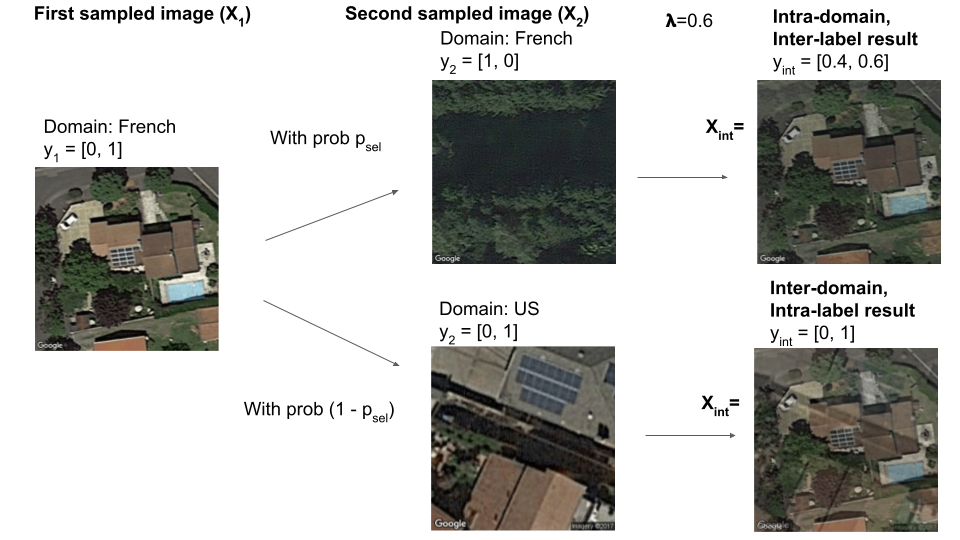
\includegraphics[width=.7\linewidth]{lisa_viz.png}  
\captionsetup{justification=centering,margin=0cm}
\caption{Diagram showing one step of LISA data augmentation.}
\label{fig:lisa}
\end{figure*}

\section{Dataset and Features}

We make use of two satellite imagery datasets for this project: (1) the original Deepsolar United States dataset, published in 2017 \cite{DeepSolar1}, and (2) a recently published dataset for France (released January 2023) \cite{Kasmi2023}.  

\begin{figure}[htp]
\centering
\begin{subfigure}{.2\textwidth}
    \centering
    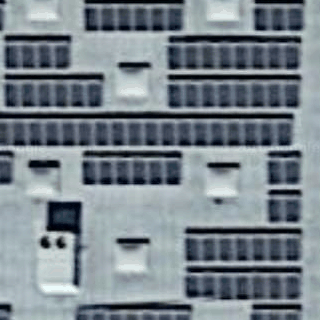
\includegraphics[width=.95\linewidth]{img_usa.png}  
    \caption{USA example}
    % \label{Raw image}
\end{subfigure}
\begin{subfigure}{.2\textwidth}
    \centering
    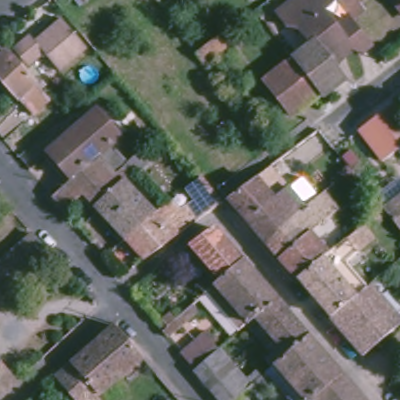
\includegraphics[width=.95\linewidth]{img_french.png}  
    \caption{French example}
    % \label{CAM segmentation}
\end{subfigure}
\captionsetup{justification=centering,margin=0cm}
\caption{Example images from our datasets}
\label{fig:datasets}
\end{figure}

The United States dataset is large and highly skewed. It includes 46,090 images with solar panels (positive) and 366,467 images without solar panels (negative). For positive images, we also have access to masks with 1 and 0 pixels indicating exactly where in the image the solar panel lies. The dataset covers industrial and residential regions of the country. The resolution of each of the images is 320 x 320, as can be seen in Figure \ref{fig:datasets}.  \cite{DeepSolar1}. 

 The France dataset provides ground truth segmentation masks for 13,303 images from Google Earth25 and 7,686 images from the French national Institute of Geographical and Forestry Information (IGN). These two sources have substantial overlap and so we picked just one to focus on for this paper. We choose the Google-sourced images because they had a lower ground sampling distance (GSD) 0.1 meters per pixel (versus IGN of 0.2 meters per pixel), and hence lower resolution, as well as the fact that there were a larger quantity of them. The dimension of each of the Google and IGN images is 400 x 400 and they are both 72 pixels/inch.  The data set focuses on more rural and residential regions versus the USA dataset. As can be seen in Figure \ref{fig:datasets}. \cite{Kasmi2023} 
 
 In addition to the LISA specific transforms covered in the methods section, we also applied random rotations in 90-degree increments, horizontal flips, and vertical flips. We resize the images to a standard input size of 299 $\times$ 299 and normalize the mean and standard deviation of each channel in the image for consistency as a preprocessing step. Apart from LISA, these data augmentation and preprocessing steps are the same as what was originally used for training the baseline DeepSolar model. 
 
For the new approaches, we split the French data set into evaluation (5000 images per class), validation (1000 images per class), and training sets (the remainder of the images). We then sampled from the training set to create class-balanced finetuning (training) datasets with 100, 500, 1000, and 5000 images per class, respectively. For finetuning with LISA specifically, within each finetuning/training dataset, we also include an equivalent amount of data from each class from the US training dataset for interpolation/data augmentation. We used each of the small finetuning (training) datasets and the validation set for training and hyperparameter tuning the DeepSolar model, to try the two different finetuning approaches described in the Methods section. Finally, we evaluated all of our finetuned models and the baseline original DeepSolar model using both the original US DeepSolar evaluation set, and French evaluation set.


\section{Experiments, Results, and Discussion}
\subsection{Model architecture and training pipeline}
The DeepSolar model \cite{DeepSolar1} consists of an Inception3 model for classification of images as containing a solar panel or not as the main backbone of the model. The auxiliary segmentation branch takes intermediate outputs of the Inception3 model as input and produces a $35 \times 35$ class activation map (CAM) as output. The CAM can be used to estimate the total area of solar panels in the image if the classification branch predicts positive. The segmentation branch is trained in a semi-supervised manner with a classification objective using the same input data and labels as the classification branch training data. A diagram of the architecture is located in the Appendix 8.1.

For each method and finetuning dataset, we performed finetuning in three steps, following the original training procedure used by the Deepsolar team \cite{DeepSolar1}. This includes training the classification branch first, and then conducting greedy layer-wise training of the two-convolutional-layer segmentation branch.

\begin{enumerate}
\item Initialize the classification branch of the model with the pretrained, original DeepSolar model weights. Finetune the entire classification branch using the classification labels of the finetuning dataset.
\item Freeze the finetuned classification branch parameters, and initialize the first convolutional layer of the segmentation model from the original DeepSolar model parameters. Finetune the first convolutional layer of the segmentation branch using the classification labels of the dataset, attaching a global average pooling layer followed by a linear layer and softmax classification output to the convolutional layer. 
\item Freeze the classification branch parameters and segmentation branch's first convolutional layer, and initialize the segmentation branch's second convolutional layer using the original DeepSolar model parameters. Finetune the second convolutional layer of the segmentation branch using the same classification objective and setup as in the previous step.
\end{enumerate}

\subsection{Evaluation metrics}

The evaluation metrics we used for classification were precision, recall, and accuracy. Note that, although our training, validation, and evaluation sets from the French dataset are class-balanced, the US dataset is extremely class-imbalanced with the vast majority of samples being negative. Therefore, for metrics reported from the US dataset, accuracy is not a good measure of model performance--this is why we also utilize precision, recall, and F1 score, which are more indicative of true model performance on a skewed dataset. 

For segmentation, we calculate an Intersection over Union (IoU) metric by comparing the predicted CAMs to the true segmentation masks, which we resize to the CAM size. This estimates how well positive areas of the CAM correspond to the true segmentation masks and allows us to interpret what the model activates on when classifying an image as containing a solar panel or not. We also report predicted area error, which is defined as the difference between predicted solar panel area and true solar panel area, divided by the true solar panel area. From a practical standpoint, this metric is useful when using model predictions to estimate the total solar panel area over a large quantity of satellite images. During finetuning, we use this metric to tune the segmentation threshold hyperparameter value for each model, described in the Hyperparameter tuning section below. Therefore, although we achieve low area errors via hyperparameter tuning, the IoU metric is more useful for understanding how well the model segments images and identifies areas corresponding to solar panels specifically.

To measure robustness, we use effective robustness $\text{metric}_{er}$ and relative robustness metrics $\text{metric}_{rr}$, adapted from the effective robustness and relative robustness metrics defined by \cite{Taori2020}. The equations applied to our use case are defined below: 
% Metric effective robustness per model is calculated as: metric(model, FR dataset) - metric(model, US dataset)
% Metric relative robustness per model is calculated as: metric(finetuned model, FR dataset) - metric(original baseline model, FR dataset) 
\begin{equation}
\text{metric}_{er} = \text{metric}(f, D_{fr}) - \text{metric}(f, D_{us})
\end{equation}
\begin{equation}
\text{metric}_{rr} = \text{metric}(f_{ft}, D_{fr}) - \text{metric}(f_{bs}, D_{fr})
\end{equation} \\
Within these equations, $f$ represents a model, $f_{ft}$ represents a finetuned model, $f_{bs}$ represents the baseline original DeepSolar model, $D_{fr}$ represents the French evaluation set, $D_{us}$ represents the US evaluation set, and metric represents any metric that is scaled between 0 and 1, such as precision, recall, accuracy, or IoU. 

Metric effective robustness measures how much better the model does on the French dataset compared to the US dataset. Metric relative robustness based on the French dataset measures how much better a finetuned model does on the French dataset than the baseline DeepSolar model. Together, they indicate how well a finetuned model adjusts to the distribution shift between US and French data. Ideally, a finetuned model will have close to 0 $metric_{er}$ indicating robustness to shifts between the French and US dataset domains (equal performance on each), and positive $metric_{rr}$, indicating improved robustness to the shift from US to French data compared to the original DeepSolar baseline.


\subsection{Hyperparameter tuning}

For regularized fine-tuning, we used grid search over learning rate, learning rate decay and L2 weight regularization (weight decay). Hyperparameter sweeps were done for each step of the fine-tuning pipeline (classification branch, segmentation branch convolution layer 1, and segmentation branch convolution layer 2) separately. For LISA data augmentation, we utilized Weights and Biases' \cite{wandb} Bayesian hyperparameter tuning \cite{bayesiantuning} feature to run sweeps. The tuned parameters included learning rate, learning rate decay, L2 weight decay, $p_{sel}$. Similarly to the regularized fine-tuning model, the hyperparameter sweeps were repeated for each step of the pipeline.  

We selected hyperparameters based on the combinations that achieved the highest validation set classification accuracy. We chose to tune using the classification accuracy because our finetuning validation set is class-balanced, meaning that acccuracy provides a good overall, single-number representation of model performance. Tuning $p_{sel}$ was only done for the classification branch finetuning. After classification branches were finetuned, the segmentation layers were finetuned using the same $p_{sel}$ as the corresponding classification branch, based on the reasoning that changing $p_{sel}$ could cause a change in the training data distribution and therefore negatively impact segmentation layer finetuning. However, we overall found that $p_{sel}$ was not an important hyperparameter for tuning, and that learning rate, weight decay, and learning rate decay were much more important.

After finetuning the model with each method and finetuning dataset, we separately tuned the segmentation threshold value (between 0 and 1) for each finetuned model individually. The segmentation threshold value is used for identifying a positive pixel in the CAM produced by the segmentation branch. We select the value to the nearest hundredth's decimal place to minimize the percentage solar panel area error (described in the metrics section) predicted over the finetuning validation set. 


\subsection{Results}
Table 1 provides a summary of our key experimental results, including classification and segmentation performance metrics for our finetuned model variants on the test French dataset. We train separate models for different amounts of labeled target data to understand the "efficiency" with which a particular finetuning method adapts to the new domain (i.e. does it need 100 or 5000 data points to achieve comparable results to USA baseline). Encouragingly, we are able to achieve comparable performance across classification and segmentation to the Deepsolar Baseline on USA dataset after finetuning on just 500 samples for regularized fine-tuning (e.g. IOU of 0.48 vs 0.51). While LISA performs similarly well for classification, it never quite achieves baseline performance for segmentation (IOU of 0.40 vs 0.51), but learns more quickly from the first 100 target samples and (as we'll see from the robustness analysis) is less prone to overfitting any given new domain.

\begin{table*}[htp]
\centering
\begin{tabular}{lcccccccc}
&  & \multicolumn{1}{l}{} 
   & \multicolumn{4}{c}{\textit{Classification}}                       
   & \multicolumn{2}{c}{\textit{Segmentation}} \\ 
\hline
Model & \begin{tabular}{@{}c@{}}Eval. \\ Dataset\end{tabular} & \begin{tabular}{@{}c@{}}Finetune \\ Samples\end{tabular} & \multicolumn{1}{c}{Accuracy} & \multicolumn{1}{c}{F1 Score} & \multicolumn{1}{c}{Precision}  & \multicolumn{1}{c}{Recall} & \multicolumn{1}{c}{Area Error} & \multicolumn{1}{c}{IOU} \\ \hline
Deepsolar Baseline & USA & n/a & 0.99 & 0.91 & 0.95 & 0.86 & -0.08  & 0.51 \\
Deepsolar Baseline & France & n/a & 0.57 & 0.24 & 0.96 & 0.14 & -0.73 & 0.06 \\ 
\hline
Regularized Fine-tuning & France & 100 & 0.87 & 0.87 & 0.86 & 0.89 & 0.10 & 0.23 \\
Regularized Fine-tuning & France & 500 & 0.94 & 0.94 & 0.97 & 0.91 & -0.24 & 0.48 \\
Regularized Fine-tuning & France & 1000 & 0.97 & 0.96 & 0.96 & 0.97 & 0.10 & 0.52 \\
Regularized Fine-tuning & France & 5000 & 0.98 & 0.98 & 0.97 & 0.99 & -0.02 & 0.54 \\ 
% \hline
% Oracle + Finetuned Segmentation & France (Google) & 100 & 1.00 & 1.00 & 0.12 & 0.28 \\
% Oracle + Finetuned Segmentation & France (Google) & 500 & 1.00 & 1.00 & -0.02 & 0.51 \\
% Oracle + Finetuned Segmentation & France (Google) & 1000 & 1.00 & 1.00 & 0.79 & 0.57 \\
% Oracle + Finetuned Segmentation & France (Google) & 5000 & 1.00 & 1.00 & 0.22 & 0.54 \\ 
\hline
LISA Data Augmentation &  France  & 100 &  0.87 & 0.88 & 0.81 & 0.98 & 0.02 & 0.31 \\
% LISA Data Augmentation &  US  & 100 &  0.88 & 0.09 & 0.85 & 0.69 & 0.03 \\
LISA Data Augmentation &  France  & 500 &  0.95 & 0.95 & 0.95 & 0.96 & 0.07 & 0.40 \\
% LISA Data Augmentation &  US  & 500 &  0.98 & 0.32 & 0.79 & -0.30 & 0.1 \\
LISA Data Augmentation &  France  & 1000 &  0.97 & 0.97 & 0.96 & 0.98 & -0.04 & 0.10 \\
% LISA Data Augmentation &  US  & 1000 & 0.93 & 0.13 & 0.78 & 0.01 & 0.01 \\
LISA Data Augmentation &  France  & 5000 &  0.97 & 0.97 & 0.96 & 0.98 & -0.04 & 0.38 \\
% LISA Data Augmentation &  US  & 5000 & 0.95 & 0.16 & 0.72 & 0.60 & 0.06 \\
% \hline
% Oracle + LISA Segmentation &  France (Google)  & 100 & 1.00  &  &  &  \\
% Oracle + LISA Segmentation &  France (Google)  & 500 & 1.00 &  &  &  \\
% Oracle + LISA Segmentation &  France (Google)  & 1000 & 1.00 &  &  &  \\
% Oracle + LISA Segmentation &  France (Google)  & 5000 & 1.00 &  &  &  \\
\hline
\end{tabular}
\begin{center}
    \caption{Summary of experimental results showing performance of (1) the Deepsolar Baseline model (pretrained) on the original US dataset compared to results with the same model on the French dataset; and (2) the Regularized Fine-tuning and LISA Data Augmentation model variants trained on varying quantities of labeled data from the target (French) datatset. 
    % For each, we consider accuracy, precision and recall for the classification component, as well as area error (predicted area - true area) / true area) and intersection over union (IOU) for segmentation. We also compare US dataset results to those of the original Deepsolar US model but using Facebook's Segment Anything Model for segmentation. 
    Accuracy, Precision and Recall are all based on the image classification performance of the model. Area error measures the relative difference between the predicted solar PV area and the true solar PV area as measured by the true segmentation masks. IOU stands for intersection over union which is our primary measure of correctness for the segmentation task.}
\end{center}
\label{table:results}
\end{table*}

Figure \ref{fig:convergence} visualizes how the performance of our two models changes as we increase the amount of available labeled target data across different metrics. As hoped, for classification accuracy we see a diminishing returns curve, with minimal uplift after 1000 data points. The story for segmentation is a bit messier. For relative area error, we quickly are able to achieve very good accuracy with minimal finetuning and so the differences after 100 data points are small and within margin of statistical noise. For IOU, both models again exhibit a diminshing retruns curve, notably with LISA outperforming Regluarized Finetuning for fewer labeled data points but converging asymptotically to a lower score. (For clarity we have removed the LISA IOU score for 1000 target data samples since we had signficiant trouble fitting this model as reflected by results in table 1.) 

\begin{figure*}[htp]
\centering
\begin{subfigure}{.3\textwidth}
    \centering
    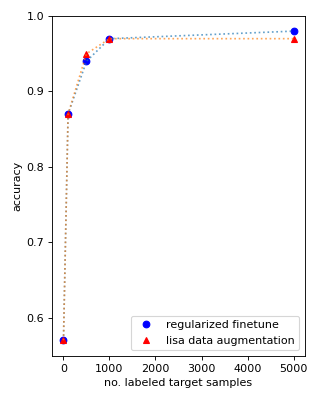
\includegraphics[width=.95\linewidth]{y_acc.png}  
    \caption{Accuracy}
    % \label{Raw image}
\end{subfigure}
\begin{subfigure}{.3\textwidth}
    \centering
    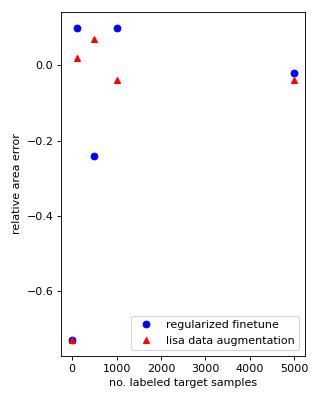
\includegraphics[width=.95\linewidth]{y_area.png}  
    \caption{Relative Area Error}
    % \label{CAM segmentation}
\end{subfigure}
\begin{subfigure}{.3\textwidth}
    \centering
    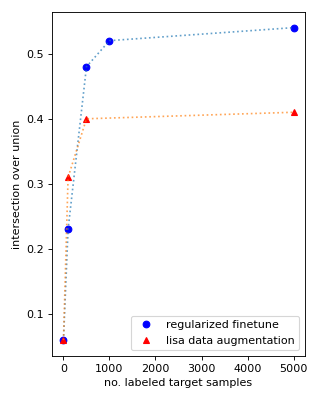
\includegraphics[width=.95\linewidth]{y_iou.png}  
    \caption{Intersection over Union}
    % \label{True segmentation}
\end{subfigure}
\caption{Compares convergence of both models across several key metrics as we increase available labeled target data.}
\label{fig:convergence}
\end{figure*}


Table 2 results examine the ability of our models to generalize between the two datasets (domains). For classification, our finetuned models achieve good Relative Robustness (RR, want > 0)  but poor Effective Robustness (ER, want $\approx$ 0). This suggests that while we have demonstrated our regularized fine-tuning and LISA data augmentation techniques can be finetune effectively (and efficiently) to new domains, we have not achieved a "robust" model that can handle multiple difference domains at once. One nuance is that our LISA model's ER (0.72 to 0.71) and RR (0.64 to 0.73) do not worsen as we increase the amount of label target samples we use for finetuning. This is an advantage of LISA over the regularized fine-tuning method for extrapolating to other domains without available labeled data. Note, we choose to use F1 score for this analysis since it combines precision and recall into one easy-to-compare metric and excludes accuracy which is misleading given the imbalance of the USA dataset (i.e. our French evaluation set is 50:50 while the USA dataset is 1:99 positive to negative samples). 

The story is similar for segmentation. Again we achieve good RR results across both models suggesting we have done a good job of adjusting to the French domain, but the ER results are still poor and confirm we probably cannot use these models without some minimal finetuning on new domains. We also observe that the LISA model's ER (0.28 to 0.32) and RR (0.25 to 0.32) hold up even as we increase the amount of target data used for finetuning, whereas regularized fine-tuning sees ER worsen significantly (0.20 to 0.52!). Note, we choose to use IOU for this analysis since it is a more precise (and less noisy) measure the quality of our segmentation task than relative area error.

% Metric effective robustness per model is calculated as: metric(model, FR dataset) - metric(model, US dataset)
% Metric relative robustness per model is calculated as: metric(finetuned model, FR dataset) - metric(original baseline model, FR dataset) 
\begin{table*}[htp]
\centering
\begin{tabular}{lccccccccc}
&  & \multicolumn{4}{c}{Classification: F1 Score} & \multicolumn{4}{c}{Segmentation: IOU} \\ \hline
Model & \begin{tabular}{@{}c@{}}Finetune \\ Samples\end{tabular} & F1(US) & F1(Fr) & ER & RR & IOU(US) & IOU(Fr) & ER & RR \\ 
\hline
Deepsolar Baseline & n/a & 0.91 & 0.24 & -0.67 & n/a & 0.51 & 0.06 & -0.45 & n/a \\ 
\hline
Regularized Fine-tuning & 100 & 0.22 & 0.87 & 0.65 & 0.63 & 0.03 & 0.23 & 0.20 & 0.17 \\
Regularized Fine-tuning & 5000 & 0.06 & 0.98 & 0.92 & 0.74 & 0.02 & 0.54 & 0.52 & 0.48 \\ 
\hline
LISA Data Augmentation & 100 & 0.16 & 0.88 & 0.72 & 0.64 & 0.03 & 0.31 & 0.28 & 0.25 \\
LISA Data Augmentation & 5000 & 0.26 & 0.97 & 0.71 & 0.73 & 0.06 & 0.38 & 0.32 & 0.32 \\ 
\hline
\end{tabular}
\begin{center}
    \caption{Calculates "robustness distribution shift" metrics suggested by \cite{Taori2020}, including Effective Robustness (ER) and Relative Robustness (RR). We show these results for classification F1 score and segmentation IOU for Deepsolar Baseline, Regularized Fine-tuning and LISA Data Augmentation models at 100 and 5000 labeled target data samples.}
\end{center}
\label{table:robust}
\end{table*}

\subsection{Error Analysis and Examples}
For cases where our classification accuracy was below 90\% (i.e. when only 100 labeled target data samples used for finetuning) we wanted to understand the effect of our improvements made to the segmentation component independent of classification performance. To do this, we used an "oracle technique" whereby we fed the correct classification (labels) into the segmentation model and measured the difference in Area Error and IOU. We find that while the difference is negligible for finetuning with 500 or more labeled target samples, the difference is meaningful for IOU when only exposed to 100 samples from target distribution (0.23 vs 0.28 and 0.31 vs 0.38). This matches our intuition that the classifier performance has a significant flow through impact on segmentation. This is particularly true for recall (otherwise segmentation model never gets a chance to predict pixels!) and helps to explain why LISA outperformed regularized fine-tuning in the 100 data samples scenario. Interestingly, we did not observe this relationship for Area Error, however, this was overall a much noisier (and low overall error) metric.

\begin{table}[htp]
\begin{tabular}{lcccc}
& \multicolumn{2}{c}{Area Error} & \multicolumn{2}{c}{IOU} \\ 
\hline
Model  & Classifier & Oracle  & Classifier & Oracle \\ 
\hline
RF  & 0.10  & 0.12   & 0.23  & 0.28   \\
LISA & 0.02  & -0.19  & 0.31  & 0.38  \\ 
\hline
\end{tabular}
\caption{Comparing segmentation metrics (Area Error, IOU) for Regularized Fine-tuning and LISA Data Augmentation models when we use an oracle vs trained classifier as input. All experiments in this table as for finetuning with 100 labeled target samples.}
\label{table:oracle}
\end{table}

Figure \ref{fig:examples} shows five illustrative examples of where our models succeed and fail for segmentation. The first two rows capture the main difference between the original Deepsolar Baseline and our fintuned model variants: misclassification of images flowing through to poor segmentation. Our baseline model, for example, achieved precision of 0.96 but recall of only 0.14. This means it was confident in the images it did select but misclassified a bunch of images that did in fact have solar panels. For those images, it predicted an empty segmentation! This clearly flows through to our baseline segmentation results where we significantly underpredict total area (-73\%) and achieve only 0.06 IOU. 

The subsequent three rows in Figure \ref{fig:examples} show more nuanced cases where we succeed and fail. Our largest sources of error remaining in the regularized fine-tuning and LISA data augmentation models were due to diffuse prediction (row 3) and object confusion (row 4). As we add more data from the French dataset which is more heavily weighted towards residential settings, our models improved at correctly identifying objects (e.g. row 5 where we no longer confuse a swimming pool for a solar panel) but do not improve much in terms of diffuse prediction error (coloring in panel plus remaining roof space). 

To address diffuse prediction error, we also tried tuning our CAM segmentation threshold (how confident do we need to be for a pixel to be considered 1 vs 0) as an additional hyperparameter. This made a significant difference for relative total area error but we found negligible uplift for IOU since our model will often put comparable weight on panel and roof so we could easily be eliminating some of the true pixels as we remove false pixels.

\begin{figure*}[htp]
\centering
\title{Illustrative example segmentation results on France test image data}
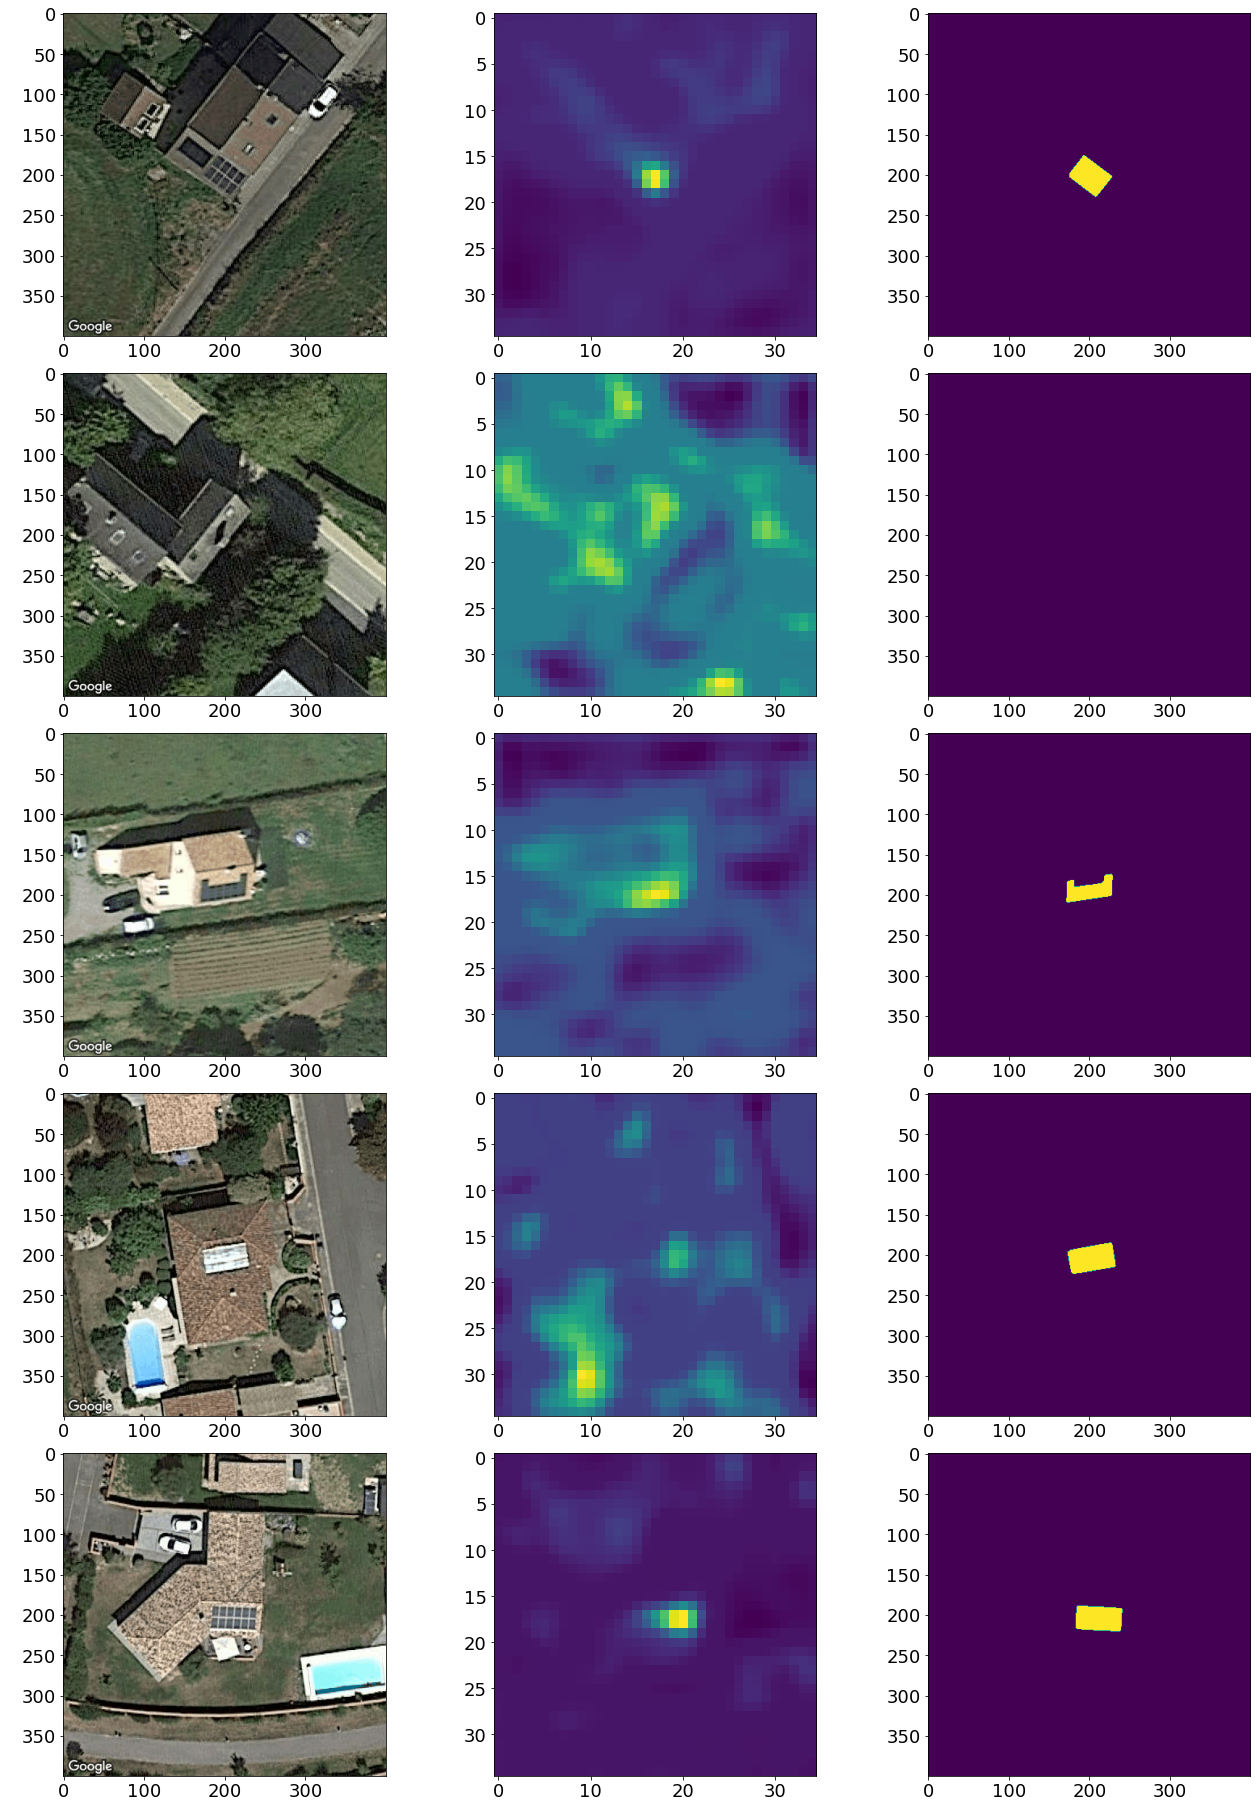
\includegraphics[width=.85\linewidth]{final/good_bad_examples.png}  
\caption{Columns: original input image (left), CAM activations from Regularized Fine-tuning model (middle), and true segmentation masks (right). Rows: (1) good example of a simple one panel segmentation; (2) bad example of model misclassification; (3) bad example of overly diffuse prediction; (4) bad example of confusing panel for another object in the scene; (5) good example of correctly ignoring that same object (backyard swimming pool).}
\label{fig:examples}
\end{figure*}

% \begin{figure*}[htp]
% \centering
% \begin{subfigure}{.3\textwidth}
%     \centering
%     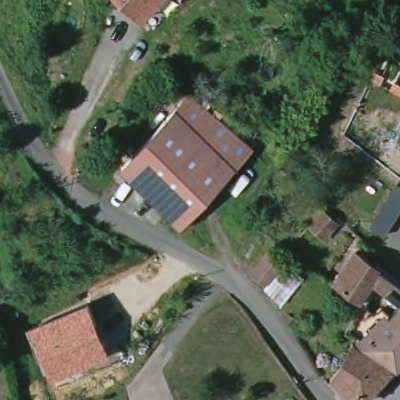
\includegraphics[width=.95\linewidth]{example.png}  
%     \caption{Raw image}
%     % \label{Raw image}
% \end{subfigure}
% \begin{subfigure}{.3\textwidth}
%     \centering
%     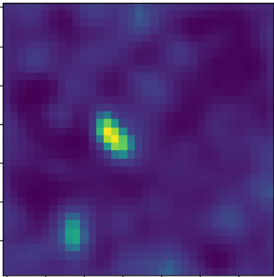
\includegraphics[width=.95\linewidth]{example_cam_seg.png}  
%     \caption{CAM segmentation}
%     % \label{CAM segmentation}
% \end{subfigure}
% \begin{subfigure}{.3\textwidth}
%     \centering
%     
\includegraphics[width=.95\linewidth]{example_true_seg.png}  
%     \caption{True segmentation}
%     % \label{True segmentation}
% \end{subfigure}
% \caption{Example result from DeepSolar baseline model trained on United States data and asked to predict segmentation masks of France test image data. True segmentation masks (rightmost), CAM activations from the original DeepSolar model (middle), and the original input image (leftmost).}
% \label{FIGURE LABEL}
% \end{figure*}



\section{Conclusion}

In conclusion, this paper presented an analysis of the DeepSolar model's performance on aerial imagery datasets from the United States and France. Deepsolar suffers significant performance loss when evaluated on the French dataset, with classification F1 score falling from 0.91 to 0.24 and segmentation IOU falling from 0.51 to 0.06. To overcome the distribution shift between the United States and France datasets, two approaches were explored: regularized fine-tuning and LISA data augmentation. 
% Regularized fine-tuning prevents rapid divergence from the pre-trained weights by incorporating L2 regularization with a tuned weight decay constant. LISA data augmentation employs linear interpolation between training examples from different distributions and with different labels to improve model robustness to distribution shifts.

We find both approaches achieved comparable classification performance to Deepsolar on the US dataset after training on just 500 samples (F1 scores of 0.94 and 0.95 vs Deepsolar's 0.91). Similarly for segmentation, both models demonstrated significant uplift after 500 samples (IOU of 0.48 and 0.40 vs Deepsolar's 0.51). While these results confirm we are able to effectively (and efficiently) finetune our original model weights for the new French dataset, an analysis of robustness metrics suggests that our model variants are unlikely to generalize to new domains without at least some minimal fine-tuning. 
% This study contributes to understanding the challenges and potential solutions for adapting the DeepSolar model to different datasets. The findings highlight the advantages and limitations of fine-tuning techniques and data augmentation strategies for achieving robustness to distribution shifts.

\section{Future Work}

Future work should include expand this investigation to include additional known distribution shift techniques such as Domain Adaptation and General Adversarial Networks (GANs). It would also be interesting to investigate if choosing a lower $p_{sel}$ value when finetuning with LISA could improve model robustness to distribution shifts, because a lower $p_{sel}$ value encourages using more diverse domain samples during finetuning--although we tuned $p_{sel}$ within this project, we tuned to maximize performance on the French dataset rather than for model robustness metrics. 

\newpage
\section{Appendices}
\subsection{Deepsolar Model Architecture}
See Figure \ref{fig:architecture} for Deepsolar model architecture, including Inception3 classification and two levels of segmentation. 
\begin{figure*}[htp]
\centering
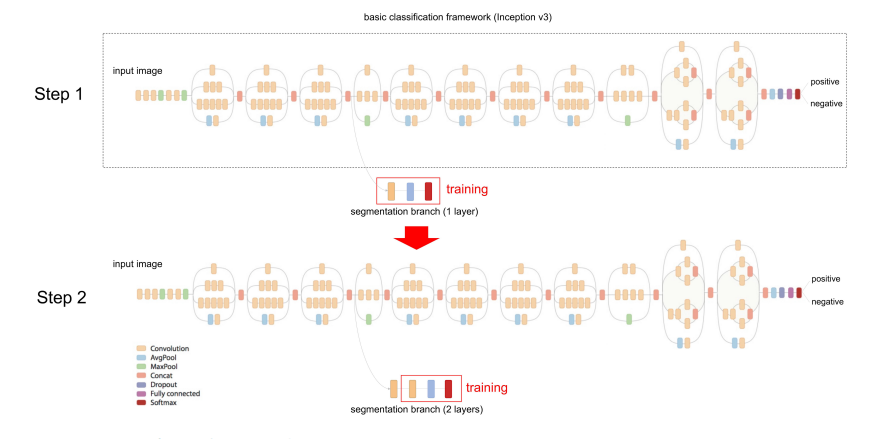
\includegraphics[width=15cm]{inception3.png}
\caption{The layers in the dashed box form the basic classification framework (Inception-v3 model). Greedy layer-wise training is performed in two steps (labelled in the left in the figure). Step 1: Keep all layers fixed but train a single “convolutional layer-GAP-linear classifier” structure in the segmentation branch. Step 2: Add another “convolutional layer-GAP-linear classifier” structure at the end of the segmentation branch and train it with all other layers fixed.\cite{DeepSolar1}}
\label{fig:architecture}
\end{figure*}

\subsection{Segment Anything Model}
During the first month of the project we experimented with Facebook's newly released Segment Anything Model (SAM) \cite{kirillov2023segment}. This was a suggestion by the Deepsolar team to see if we could boost segmentation performance on the original USA dataset. Our initial experiments did show some promise! By randomly sampling three positive and three negative points from our predicted segmentation CAM and passing these as prompts to the SAM model, we were able to achieve 0.47 relative area error and 0.24 IOU. We ultimately choose to focus our attention on the distribution shift problem since we were more excited about it's potential use cases beyond this course, but would suggest there is certainly further potential in designing more sophisticated prompts to improve the Deepsolar + SAM segmentation results.  

\begin{figure*}[htp]
\centering
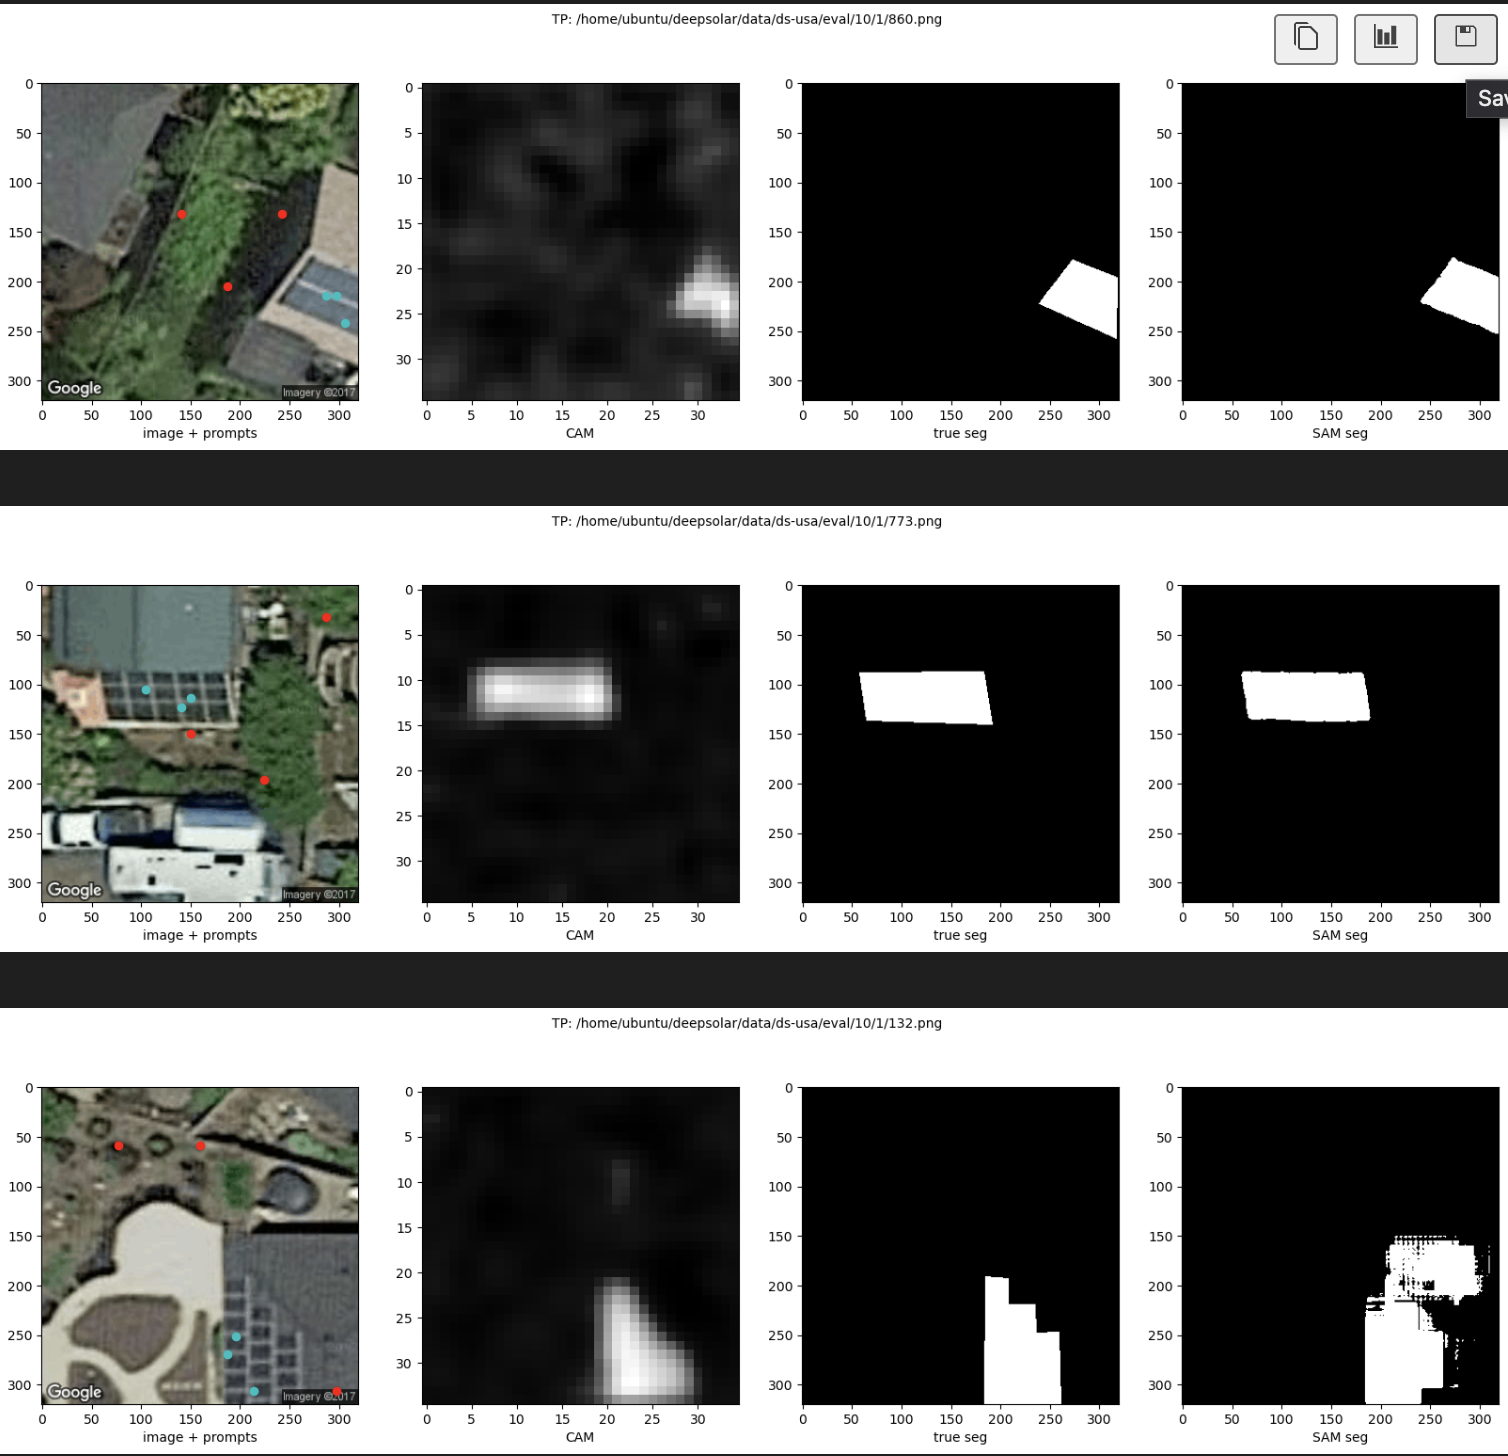
\includegraphics[width=15cm]{prelim_sam.png}
\caption{Preliminary segmentation of solar PV cells with SAM (rightmost column), compared to true segmentation masks (second from right), CAM activations from the original DeepSolar model (third from right), and the original input image (leftmost) with positive point prompts in cyan, and negative point prompts in red.}
\end{figure*}

\subsection{Generative Adversarial Network}
We also experimented with developing a Generative Adversarial Network (GAN) to enhance the training data for the satellite imagery models based on some of the recommendations in \cite{volpi2018generalizing}. The objective was to create a more robust and accurate model by augmenting the training examples with challenging samples.

At each iteration of the training process, we tried to incorporate difficult examples that were specifically chosen to challenge the current model. This approach aimed to improve the model's ability to handle complex and diverse scenarios, ultimately leading to better performance on the distribution shift issues experienced by the Deepsolar model between the French and the USA datasets.

While experimenting on AWS, after the first iteration, the Discriminator (D) and Generator (G) losses were measured at 1.385 and 0.5776, respectively. This indicated that the model was learning and making progress towards achieving the desired outcome.

Unfortunately, the process was interrupted or terminated after this initial iteration, resulting in incomplete results.  Further analysis and experimentation are needed to draw definitive conclusions about the effectiveness of this approach for the Deepsolar model, and so we recommend this larger body of research for future work.



\newpage
\section{Contributions and Acknowledgements}
Github code repository for this project can be accessed at https://github.com/jelc53/deepsolar.git \\

Contributions: Kerrie owned development of the LISA data augmentation model implementation and experimented with SAM applications. Julian owned development of the regularized fine-tuning model implementation and experimented with GAN applications. Andrea led the literature review, owned data processing pipeling for the French dataset, and experimented with GAN applications. Everyone contributed to the model setup, running experiments on AWS server, and brainstorming design choices. \\

Acknowledgements: We would like to thank Zhecheng Wang for guidance on initial directions for the project, introducing us to DeepSolar Github repositories that we built upon, and providing us the original DeepSolar US dataset.



%%%%%%%%% REFERENCES
\newpage
{\small
\bibliographystyle{ieee_fullname}
\bibliography{egbib}
}

\end{document}
